\subsubsection{算法设计}

\paragraph{模型建立} 设目标中心为$x=0,y=0$,圆形区域半径为$a=100$,则圆形区域可表示为$\Omega: x^2 + y^2 = a^2$,炮弹的落点服从二维正态分布$N(\boldsymbol{\mu}, \boldsymbol{\Sigma})$,其中,
\begin{equation}
    \boldsymbol{\mu} = \left(\begin{matrix}
        0\\
        0
    \end{matrix}\right)
    , \quad 
    \boldsymbol{\Sigma}  = \left(\begin{matrix}
        \sigma_x^2 & r \sigma_x \sigma_y \\
        r \sigma_x \sigma_y & \sigma_y^2
    \end{matrix}\right)
\end{equation}

记$\boldsymbol{x} = (x,y)^T$,其维度$m=2$,则概率密度函数如下,图像如\Cref{fig:ex5_pdf}。
\begin{equation}
    f(\boldsymbol{x})=\left(\frac{1}{2 \pi}\right)^{\frac{m}{2}} \frac{1}{\sqrt{|\boldsymbol{\Sigma|}}} \exp \left[-\frac{1}{2}(\boldsymbol{x}-\boldsymbol{\mu})^{T} \boldsymbol{\Sigma}^{-1}(\boldsymbol{x}-\boldsymbol{\mu})\right]
\end{equation}

炮弹命中圆形区域内部的概率$p$为,
\begin{equation}\label{eq:ex5_model}
    p = \iint_\Omega f(x,y) dxdy
\end{equation}

\Cref{eq:ex5_model}即为本题的模型。

\begin{figure}[H]
    \centering
    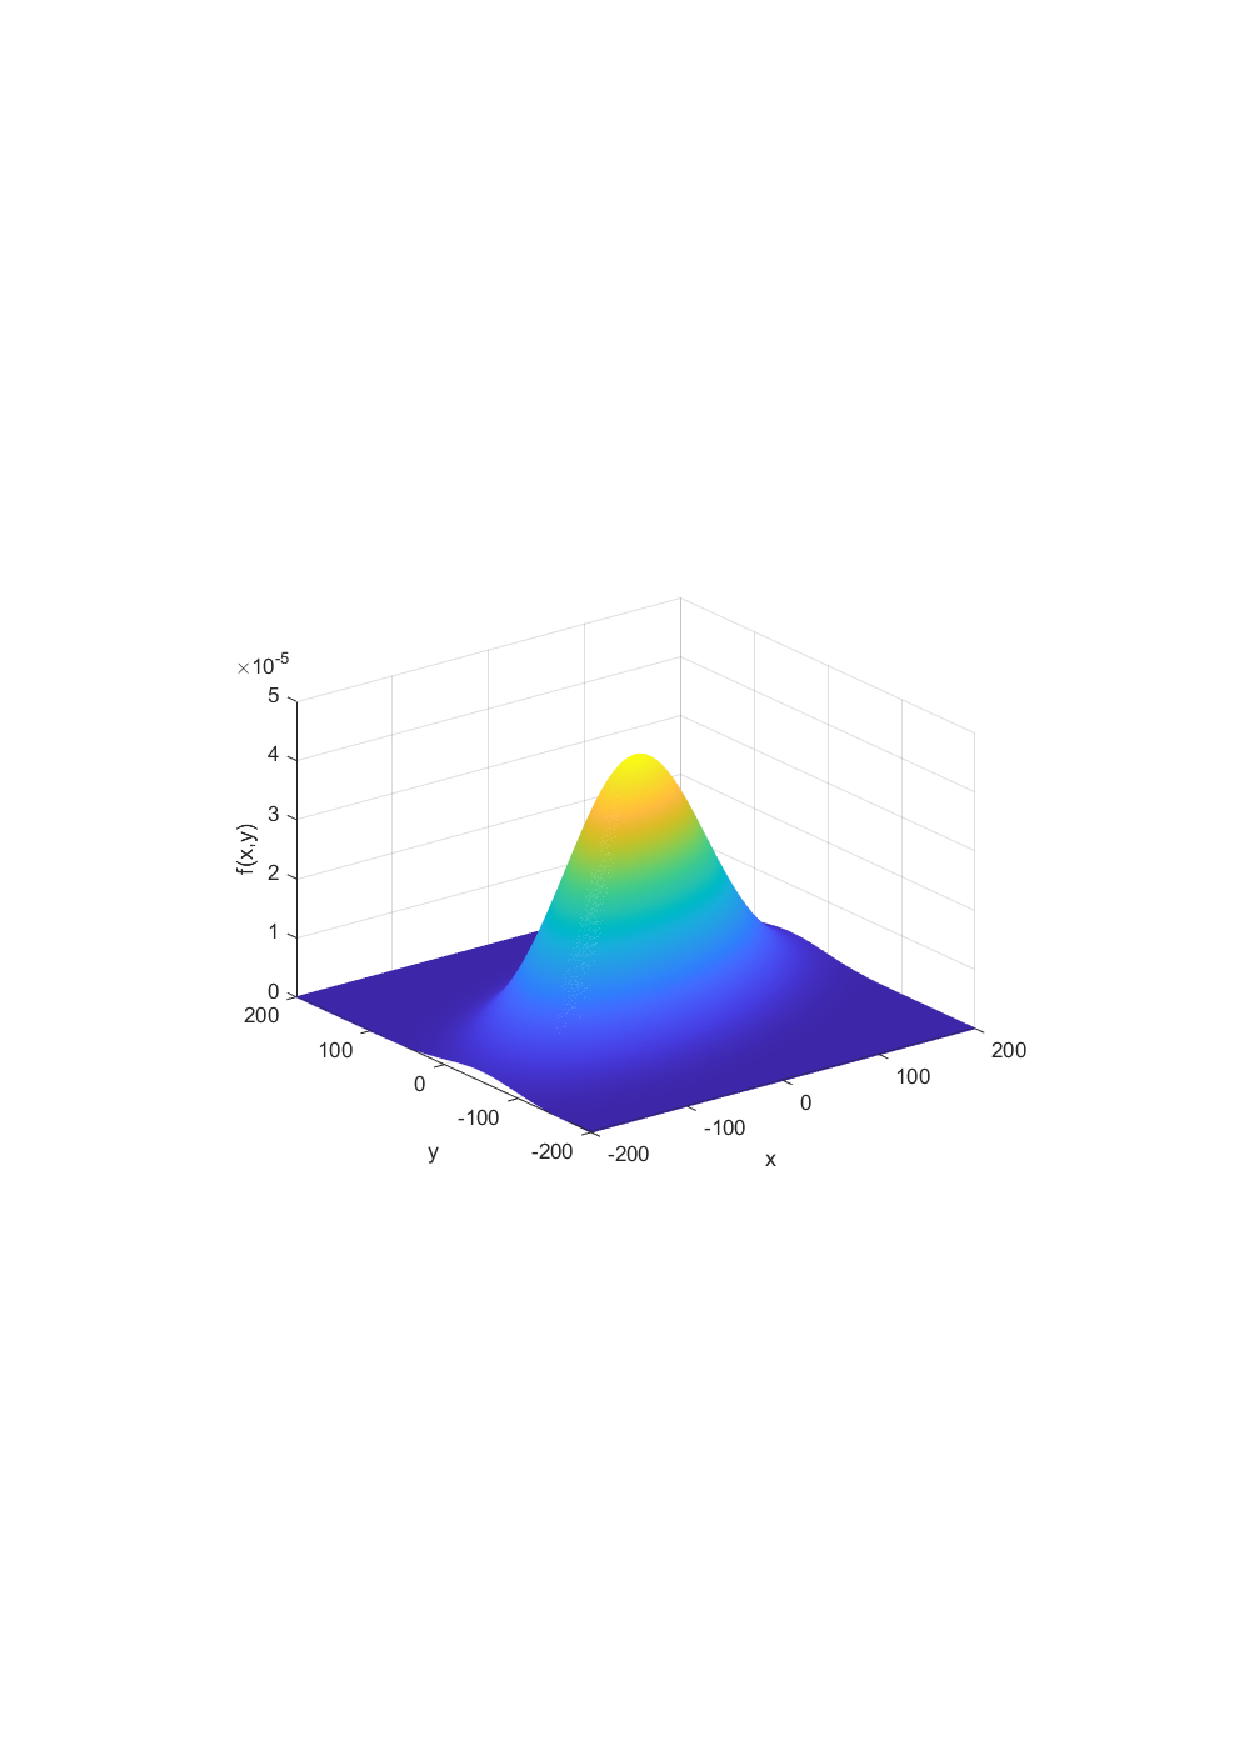
\includegraphics[width=0.8\textwidth,trim={3.09cm 9.295cm 3.09cm 9.295cm},clip]{fig/ex5_pdf.pdf}
    \caption{概率密度函数$f(x,y)$的图像}
    \label{fig:ex5_pdf}
\end{figure}

\paragraph{算法实现} 考虑到\Cref{eq:ex5_model}的二重积分无解析解,可以采用两种方法求解。

一种方法是采用蒙特卡洛方法求解,取$n$个独立均匀分布在区域$[-a,a]\times [-a,a]$的随机点$\{(x_i,y_i)\}_{i=1}^n$,记$I$为示性函数,则可近似计算得出,
\begin{equation}
    p = \frac{4a^2}{n} \sum_{i=1}^n f(x_i, y_i) I_{(x_i, y_i) \in \Omega}
\end{equation}

另一种方法是采用数值积分方法求解,即,
\begin{equation}
    p = \int_{-a}^a \int_{-a}^a f(x,y) I_{(x, y) \in \Omega} dxdy
\end{equation}

在MATLAB的实现中,可采用\texttt{mvnpdf}命令计算二维正态分布的概率密度函数$f$,采用\texttt{unifrnd}命令生成独立均匀分布的随机数,采用\texttt{integral2}命令计算二维数值积分。

\subsubsection{程序}

请参见附录\ref{sec:ex5_code}。

\subsubsection{计算结果}

\paragraph{蒙特卡洛方法} 分别选取$n=10^4,10^5,10^6,10^7$,在每个$n$值下计算5次,得到结果如\Cref{tab:ex5_results}。取$n=10^7$时5次计算的均值作为最终结果,得到$p=0.6980$。

\begin{table}[H]
    \centering
    \caption{不同$n$取值下计算5次得到的概率$p$值}
    \label{tab:ex5_results}
    \begin{tabular}{c|ccccc|cc}
        \toprule
        $n$ & 1 & 2 & 3 & 4 & 5 & Mean & Variance\tabularnewline
        \midrule
        $10^4$ & 0.7032 & 0.7030 & 0.6991 & 0.6903 & 0.7019 & 0.6995 & $2.9125\times 10^{-5}$\tabularnewline
        $10^5$ & 0.6977 & 0.6962 & 0.6970 & 0.6978 & 0.7014 & 0.6980 & $3.9820\times 10^{-6}$\tabularnewline
        $10^6$ & 0.6973 & 0.6985 & 0.6978 & 0.6979 & 0.6986 & 0.6980 & $2.8700\times 10^{-7}$\tabularnewline
        $10^7$ & 0.6980 & 0.6981 & 0.6977 & 0.6979 & 0.6984 & 0.6980 & $6.7000\times 10^{-8}$\tabularnewline
        \bottomrule
    \end{tabular}
\end{table}

\paragraph{数值积分方法} 利用数值积分方法求出的值为$p=0.6980$。

\subsubsection{结果分析}

从\Cref{tab:ex5_results}可以看出,采用蒙特卡洛方法时,随着试验次数$n$的增大,计算结果的方差逐渐减小,逐步稳定在真值附近,当$n$达到$10^5$时,蒙特卡洛结果与数值积分结果已经非常接近,可作为真值的一个近似解。

\subsubsection{结论}

炮弹命中圆形区域的概率为69.80\%。
